% Generated by ArticleSignalDiagrams. Opaque vector fills only.
\documentclass[10pt,tikz,border=5pt]{standalone}
\usepackage{lmodern}
\usetikzlibrary{fit}
\begin{document}
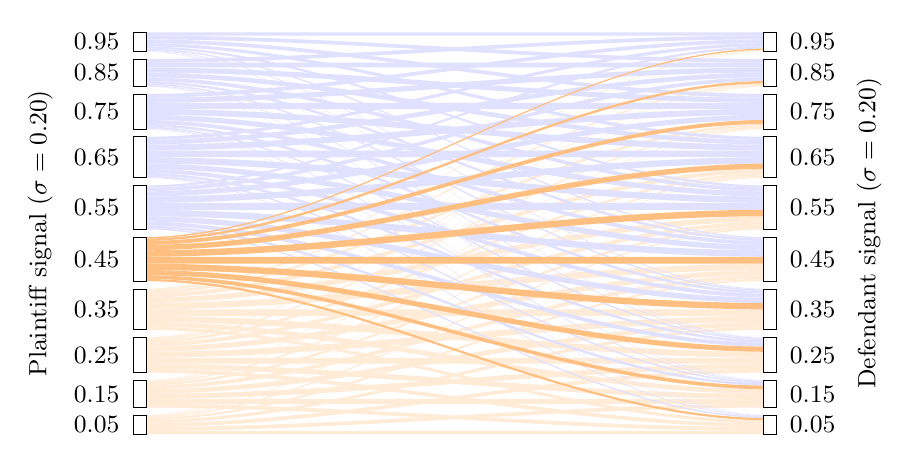
\begin{tikzpicture}[x=1cm,y=1cm,font=\small]\path[fill=orange!16!white,draw=none] (3.3,-5.1) .. controls (6,-5.1) and (8.6,-5.1) .. (11.3,-5.1) -- (11.3,-5.060219) .. controls (8.6,-5.060219) and (6,-5.060219) .. (3.3,-5.060219) -- cycle;
\path[fill=orange!16!white,draw=none] (3.3,-5.060219) .. controls (6,-5.060219) and (8.6,-4.763641) .. (11.3,-4.763641) -- (11.3,-4.716027) .. controls (8.6,-4.716027) and (6,-5.012605) .. (3.3,-5.012605) -- cycle;
\path[fill=orange!16!white,draw=none] (3.3,-5.012605) .. controls (6,-5.012605) and (8.6,-4.319108) .. (11.3,-4.319108) -- (11.3,-4.271646) .. controls (8.6,-4.271646) and (6,-4.965142) .. (3.3,-4.965142) -- cycle;
\path[fill=orange!16!white,draw=none] (3.3,-4.965142) .. controls (6,-4.965142) and (8.6,-3.774843) .. (11.3,-3.774843) -- (11.3,-3.735025) .. controls (8.6,-3.735025) and (6,-4.925324) .. (3.3,-4.925324) -- cycle;
\path[fill=orange!16!white,draw=none] (3.3,-4.925324) .. controls (6,-4.925324) and (8.6,-3.156689) .. (11.3,-3.156689) -- (11.3,-3.128277) .. controls (8.6,-3.128277) and (6,-4.896911) .. (3.3,-4.896911) -- cycle;
\path[fill=orange!16!white,draw=none] (3.3,-4.896911) .. controls (6,-4.896911) and (8.6,-2.5) .. (11.3,-2.5) -- (11.3,-2.482587) .. controls (8.6,-2.482587) and (6,-4.879498) .. (3.3,-4.879498) -- cycle;
\path[fill=orange!16!white,draw=none] (3.3,-4.879498) .. controls (6,-4.879498) and (8.6,-1.843311) .. (11.3,-1.843311) -- (11.3,-1.834069) .. controls (8.6,-1.834069) and (6,-4.870256) .. (3.3,-4.870256) -- cycle;
\path[fill=orange!16!white,draw=none] (3.3,-4.870256) .. controls (6,-4.870256) and (8.6,-1.225157) .. (11.3,-1.225157) -- (11.3,-1.220883) .. controls (8.6,-1.220883) and (6,-4.865982) .. (3.3,-4.865982) -- cycle;
\path[fill=orange!16!white,draw=none] (3.3,-4.865982) .. controls (6,-4.865982) and (8.6,-0.680892) .. (11.3,-0.680892) -- (11.3,-0.679163) .. controls (8.6,-0.679163) and (6,-4.864254) .. (3.3,-4.864254) -- cycle;
\path[fill=orange!16!white,draw=none] (3.3,-4.864254) .. controls (6,-4.864254) and (8.6,-0.236359) .. (11.3,-0.236359) -- (11.3,-0.235746) .. controls (8.6,-0.235746) and (6,-4.863641) .. (3.3,-4.863641) -- cycle;
\path[fill=orange!16!white,draw=none] (3.3,-4.763641) .. controls (6,-4.763641) and (8.6,-5.060219) .. (11.3,-5.060219) -- (11.3,-5.012605) .. controls (8.6,-5.012605) and (6,-4.716027) .. (3.3,-4.716027) -- cycle;
\path[fill=orange!16!white,draw=none] (3.3,-4.716027) .. controls (6,-4.716027) and (8.6,-4.716027) .. (11.3,-4.716027) -- (11.3,-4.655396) .. controls (8.6,-4.655396) and (6,-4.655396) .. (3.3,-4.655396) -- cycle;
\path[fill=orange!16!white,draw=none] (3.3,-4.655396) .. controls (6,-4.655396) and (8.6,-4.271646) .. (11.3,-4.271646) -- (11.3,-4.206666) .. controls (8.6,-4.206666) and (6,-4.590417) .. (3.3,-4.590417) -- cycle;
\path[fill=orange!16!white,draw=none] (3.3,-4.590417) .. controls (6,-4.590417) and (8.6,-3.735025) .. (11.3,-3.735025) -- (11.3,-3.675793) .. controls (8.6,-3.675793) and (6,-4.531185) .. (3.3,-4.531185) -- cycle;
\path[fill=orange!16!white,draw=none] (3.3,-4.531185) .. controls (6,-4.531185) and (8.6,-3.128277) .. (11.3,-3.128277) -- (11.3,-3.081902) .. controls (8.6,-3.081902) and (6,-4.48481) .. (3.3,-4.48481) -- cycle;
\path[fill=orange!16!white,draw=none] (3.3,-4.48481) .. controls (6,-4.48481) and (8.6,-2.482587) .. (11.3,-2.482587) -- (11.3,-2.451142) .. controls (8.6,-2.451142) and (6,-4.453365) .. (3.3,-4.453365) -- cycle;
\path[fill=orange!16!white,draw=none] (3.3,-4.453365) .. controls (6,-4.453365) and (8.6,-1.834069) .. (11.3,-1.834069) -- (11.3,-1.815492) .. controls (8.6,-1.815492) and (6,-4.434788) .. (3.3,-4.434788) -- cycle;
\path[fill=orange!16!white,draw=none] (3.3,-4.434788) .. controls (6,-4.434788) and (8.6,-1.220883) .. (11.3,-1.220883) -- (11.3,-1.211282) .. controls (8.6,-1.211282) and (6,-4.425187) .. (3.3,-4.425187) -- cycle;
\path[fill=orange!16!white,draw=none] (3.3,-4.425187) .. controls (6,-4.425187) and (8.6,-0.679163) .. (11.3,-0.679163) -- (11.3,-0.674813) .. controls (8.6,-0.674813) and (6,-4.420837) .. (3.3,-4.420837) -- cycle;
\path[fill=orange!16!white,draw=none] (3.3,-4.420837) .. controls (6,-4.420837) and (8.6,-0.235746) .. (11.3,-0.235746) -- (11.3,-0.234018) .. controls (8.6,-0.234018) and (6,-4.419108) .. (3.3,-4.419108) -- cycle;
\path[fill=orange!16!white,draw=none] (3.3,-4.319108) .. controls (6,-4.319108) and (8.6,-5.012605) .. (11.3,-5.012605) -- (11.3,-4.965142) .. controls (8.6,-4.965142) and (6,-4.271646) .. (3.3,-4.271646) -- cycle;
\path[fill=orange!16!white,draw=none] (3.3,-4.271646) .. controls (6,-4.271646) and (8.6,-4.655396) .. (11.3,-4.655396) -- (11.3,-4.590417) .. controls (8.6,-4.590417) and (6,-4.206666) .. (3.3,-4.206666) -- cycle;
\path[fill=orange!16!white,draw=none] (3.3,-4.206666) .. controls (6,-4.206666) and (8.6,-4.206666) .. (11.3,-4.206666) -- (11.3,-4.131001) .. controls (8.6,-4.131001) and (6,-4.131001) .. (3.3,-4.131001) -- cycle;
\path[fill=orange!16!white,draw=none] (3.3,-4.131001) .. controls (6,-4.131001) and (8.6,-3.675793) .. (11.3,-3.675793) -- (11.3,-3.600114) .. controls (8.6,-3.600114) and (6,-4.055322) .. (3.3,-4.055322) -- cycle;
\path[fill=orange!16!white,draw=none] (3.3,-4.055322) .. controls (6,-4.055322) and (8.6,-3.081902) .. (11.3,-3.081902) -- (11.3,-3.016349) .. controls (8.6,-3.016349) and (6,-3.989769) .. (3.3,-3.989769) -- cycle;
\path[fill=orange!16!white,draw=none] (3.3,-3.989769) .. controls (6,-3.989769) and (8.6,-2.451142) .. (11.3,-2.451142) -- (11.3,-2.401667) .. controls (8.6,-2.401667) and (6,-3.940294) .. (3.3,-3.940294) -- cycle;
\path[fill=orange!16!white,draw=none] (3.3,-3.940294) .. controls (6,-3.940294) and (8.6,-1.815492) .. (11.3,-1.815492) -- (11.3,-1.782825) .. controls (8.6,-1.782825) and (6,-3.907627) .. (3.3,-3.907627) -- cycle;
\path[fill=orange!16!white,draw=none] (3.3,-3.907627) .. controls (6,-3.907627) and (8.6,-1.211282) .. (11.3,-1.211282) -- (11.3,-1.192373) .. controls (8.6,-1.192373) and (6,-3.888718) .. (3.3,-3.888718) -- cycle;
\path[fill=orange!16!white,draw=none] (3.3,-3.888718) .. controls (6,-3.888718) and (8.6,-0.674813) .. (11.3,-0.674813) -- (11.3,-0.665212) .. controls (8.6,-0.665212) and (6,-3.879117) .. (3.3,-3.879117) -- cycle;
\path[fill=orange!16!white,draw=none] (3.3,-3.879117) .. controls (6,-3.879117) and (8.6,-0.234018) .. (11.3,-0.234018) -- (11.3,-0.229744) .. controls (8.6,-0.229744) and (6,-3.874843) .. (3.3,-3.874843) -- cycle;
\path[fill=orange!16!white,draw=none] (3.3,-3.774843) .. controls (6,-3.774843) and (8.6,-4.965142) .. (11.3,-4.965142) -- (11.3,-4.925324) .. controls (8.6,-4.925324) and (6,-3.735025) .. (3.3,-3.735025) -- cycle;
\path[fill=orange!16!white,draw=none] (3.3,-3.735025) .. controls (6,-3.735025) and (8.6,-4.590417) .. (11.3,-4.590417) -- (11.3,-4.531185) .. controls (8.6,-4.531185) and (6,-3.675793) .. (3.3,-3.675793) -- cycle;
\path[fill=orange!16!white,draw=none] (3.3,-3.675793) .. controls (6,-3.675793) and (8.6,-4.131001) .. (11.3,-4.131001) -- (11.3,-4.055322) .. controls (8.6,-4.055322) and (6,-3.600114) .. (3.3,-3.600114) -- cycle;
\path[fill=orange!16!white,draw=none] (3.3,-3.600114) .. controls (6,-3.600114) and (8.6,-3.600114) .. (11.3,-3.600114) -- (11.3,-3.516374) .. controls (8.6,-3.516374) and (6,-3.516374) .. (3.3,-3.516374) -- cycle;
\path[fill=orange!16!white,draw=none] (3.3,-3.516374) .. controls (6,-3.516374) and (8.6,-3.016349) .. (11.3,-3.016349) -- (11.3,-2.93561) .. controls (8.6,-2.93561) and (6,-3.435635) .. (3.3,-3.435635) -- cycle;
\path[fill=orange!16!white,draw=none] (3.3,-3.435635) .. controls (6,-3.435635) and (8.6,-2.401667) .. (11.3,-2.401667) -- (11.3,-2.333565) .. controls (8.6,-2.333565) and (6,-3.367534) .. (3.3,-3.367534) -- cycle;
\path[fill=orange!16!white,draw=none] (3.3,-3.367534) .. controls (6,-3.367534) and (8.6,-1.782825) .. (11.3,-1.782825) -- (11.3,-1.732466) .. controls (8.6,-1.732466) and (6,-3.317175) .. (3.3,-3.317175) -- cycle;
\path[fill=orange!16!white,draw=none] (3.3,-3.317175) .. controls (6,-3.317175) and (8.6,-1.192373) .. (11.3,-1.192373) -- (11.3,-1.159706) .. controls (8.6,-1.159706) and (6,-3.284508) .. (3.3,-3.284508) -- cycle;
\path[fill=orange!16!white,draw=none] (3.3,-3.284508) .. controls (6,-3.284508) and (8.6,-0.665212) .. (11.3,-0.665212) -- (11.3,-0.646635) .. controls (8.6,-0.646635) and (6,-3.265931) .. (3.3,-3.265931) -- cycle;
\path[fill=orange!16!white,draw=none] (3.3,-3.265931) .. controls (6,-3.265931) and (8.6,-0.229744) .. (11.3,-0.229744) -- (11.3,-0.220502) .. controls (8.6,-0.220502) and (6,-3.256689) .. (3.3,-3.256689) -- cycle;
\path[fill=blue!12!white,draw=none] (3.3,-2.5) .. controls (6,-2.5) and (8.6,-4.896911) .. (11.3,-4.896911) -- (11.3,-4.879498) .. controls (8.6,-4.879498) and (6,-2.482587) .. (3.3,-2.482587) -- cycle;
\path[fill=blue!12!white,draw=none] (3.3,-2.482587) .. controls (6,-2.482587) and (8.6,-4.48481) .. (11.3,-4.48481) -- (11.3,-4.453365) .. controls (8.6,-4.453365) and (6,-2.451142) .. (3.3,-2.451142) -- cycle;
\path[fill=blue!12!white,draw=none] (3.3,-2.451142) .. controls (6,-2.451142) and (8.6,-3.989769) .. (11.3,-3.989769) -- (11.3,-3.940294) .. controls (8.6,-3.940294) and (6,-2.401667) .. (3.3,-2.401667) -- cycle;
\path[fill=blue!12!white,draw=none] (3.3,-2.401667) .. controls (6,-2.401667) and (8.6,-3.435635) .. (11.3,-3.435635) -- (11.3,-3.367534) .. controls (8.6,-3.367534) and (6,-2.333565) .. (3.3,-2.333565) -- cycle;
\path[fill=blue!12!white,draw=none] (3.3,-2.333565) .. controls (6,-2.333565) and (8.6,-2.848614) .. (11.3,-2.848614) -- (11.3,-2.766435) .. controls (8.6,-2.766435) and (6,-2.251386) .. (3.3,-2.251386) -- cycle;
\path[fill=blue!12!white,draw=none] (3.3,-2.251386) .. controls (6,-2.251386) and (8.6,-2.251386) .. (11.3,-2.251386) -- (11.3,-2.16439) .. controls (8.6,-2.16439) and (6,-2.16439) .. (3.3,-2.16439) -- cycle;
\path[fill=blue!12!white,draw=none] (3.3,-2.16439) .. controls (6,-2.16439) and (8.6,-1.664365) .. (11.3,-1.664365) -- (11.3,-1.583626) .. controls (8.6,-1.583626) and (6,-2.083651) .. (3.3,-2.083651) -- cycle;
\path[fill=blue!12!white,draw=none] (3.3,-2.083651) .. controls (6,-2.083651) and (8.6,-1.110231) .. (11.3,-1.110231) -- (11.3,-1.044678) .. controls (8.6,-1.044678) and (6,-2.018098) .. (3.3,-2.018098) -- cycle;
\path[fill=blue!12!white,draw=none] (3.3,-2.018098) .. controls (6,-2.018098) and (8.6,-0.61519) .. (11.3,-0.61519) -- (11.3,-0.568815) .. controls (8.6,-0.568815) and (6,-1.971723) .. (3.3,-1.971723) -- cycle;
\path[fill=blue!12!white,draw=none] (3.3,-1.971723) .. controls (6,-1.971723) and (8.6,-0.203089) .. (11.3,-0.203089) -- (11.3,-0.174676) .. controls (8.6,-0.174676) and (6,-1.943311) .. (3.3,-1.943311) -- cycle;
\path[fill=blue!12!white,draw=none] (3.3,-1.843311) .. controls (6,-1.843311) and (8.6,-4.879498) .. (11.3,-4.879498) -- (11.3,-4.870256) .. controls (8.6,-4.870256) and (6,-1.834069) .. (3.3,-1.834069) -- cycle;
\path[fill=blue!12!white,draw=none] (3.3,-1.834069) .. controls (6,-1.834069) and (8.6,-4.453365) .. (11.3,-4.453365) -- (11.3,-4.434788) .. controls (8.6,-4.434788) and (6,-1.815492) .. (3.3,-1.815492) -- cycle;
\path[fill=blue!12!white,draw=none] (3.3,-1.815492) .. controls (6,-1.815492) and (8.6,-3.940294) .. (11.3,-3.940294) -- (11.3,-3.907627) .. controls (8.6,-3.907627) and (6,-1.782825) .. (3.3,-1.782825) -- cycle;
\path[fill=blue!12!white,draw=none] (3.3,-1.782825) .. controls (6,-1.782825) and (8.6,-3.367534) .. (11.3,-3.367534) -- (11.3,-3.317175) .. controls (8.6,-3.317175) and (6,-1.732466) .. (3.3,-1.732466) -- cycle;
\path[fill=blue!12!white,draw=none] (3.3,-1.732466) .. controls (6,-1.732466) and (8.6,-2.766435) .. (11.3,-2.766435) -- (11.3,-2.698333) .. controls (8.6,-2.698333) and (6,-1.664365) .. (3.3,-1.664365) -- cycle;
\path[fill=blue!12!white,draw=none] (3.3,-1.664365) .. controls (6,-1.664365) and (8.6,-2.16439) .. (11.3,-2.16439) -- (11.3,-2.083651) .. controls (8.6,-2.083651) and (6,-1.583626) .. (3.3,-1.583626) -- cycle;
\path[fill=blue!12!white,draw=none] (3.3,-1.583626) .. controls (6,-1.583626) and (8.6,-1.583626) .. (11.3,-1.583626) -- (11.3,-1.499886) .. controls (8.6,-1.499886) and (6,-1.499886) .. (3.3,-1.499886) -- cycle;
\path[fill=blue!12!white,draw=none] (3.3,-1.499886) .. controls (6,-1.499886) and (8.6,-1.044678) .. (11.3,-1.044678) -- (11.3,-0.968999) .. controls (8.6,-0.968999) and (6,-1.424207) .. (3.3,-1.424207) -- cycle;
\path[fill=blue!12!white,draw=none] (3.3,-1.424207) .. controls (6,-1.424207) and (8.6,-0.568815) .. (11.3,-0.568815) -- (11.3,-0.509583) .. controls (8.6,-0.509583) and (6,-1.364975) .. (3.3,-1.364975) -- cycle;
\path[fill=blue!12!white,draw=none] (3.3,-1.364975) .. controls (6,-1.364975) and (8.6,-0.174676) .. (11.3,-0.174676) -- (11.3,-0.134858) .. controls (8.6,-0.134858) and (6,-1.325157) .. (3.3,-1.325157) -- cycle;
\path[fill=blue!12!white,draw=none] (3.3,-1.225157) .. controls (6,-1.225157) and (8.6,-4.870256) .. (11.3,-4.870256) -- (11.3,-4.865982) .. controls (8.6,-4.865982) and (6,-1.220883) .. (3.3,-1.220883) -- cycle;
\path[fill=blue!12!white,draw=none] (3.3,-1.220883) .. controls (6,-1.220883) and (8.6,-4.434788) .. (11.3,-4.434788) -- (11.3,-4.425187) .. controls (8.6,-4.425187) and (6,-1.211282) .. (3.3,-1.211282) -- cycle;
\path[fill=blue!12!white,draw=none] (3.3,-1.211282) .. controls (6,-1.211282) and (8.6,-3.907627) .. (11.3,-3.907627) -- (11.3,-3.888718) .. controls (8.6,-3.888718) and (6,-1.192373) .. (3.3,-1.192373) -- cycle;
\path[fill=blue!12!white,draw=none] (3.3,-1.192373) .. controls (6,-1.192373) and (8.6,-3.317175) .. (11.3,-3.317175) -- (11.3,-3.284508) .. controls (8.6,-3.284508) and (6,-1.159706) .. (3.3,-1.159706) -- cycle;
\path[fill=blue!12!white,draw=none] (3.3,-1.159706) .. controls (6,-1.159706) and (8.6,-2.698333) .. (11.3,-2.698333) -- (11.3,-2.648858) .. controls (8.6,-2.648858) and (6,-1.110231) .. (3.3,-1.110231) -- cycle;
\path[fill=blue!12!white,draw=none] (3.3,-1.110231) .. controls (6,-1.110231) and (8.6,-2.083651) .. (11.3,-2.083651) -- (11.3,-2.018098) .. controls (8.6,-2.018098) and (6,-1.044678) .. (3.3,-1.044678) -- cycle;
\path[fill=blue!12!white,draw=none] (3.3,-1.044678) .. controls (6,-1.044678) and (8.6,-1.499886) .. (11.3,-1.499886) -- (11.3,-1.424207) .. controls (8.6,-1.424207) and (6,-0.968999) .. (3.3,-0.968999) -- cycle;
\path[fill=blue!12!white,draw=none] (3.3,-0.968999) .. controls (6,-0.968999) and (8.6,-0.968999) .. (11.3,-0.968999) -- (11.3,-0.893334) .. controls (8.6,-0.893334) and (6,-0.893334) .. (3.3,-0.893334) -- cycle;
\path[fill=blue!12!white,draw=none] (3.3,-0.893334) .. controls (6,-0.893334) and (8.6,-0.509583) .. (11.3,-0.509583) -- (11.3,-0.444604) .. controls (8.6,-0.444604) and (6,-0.828354) .. (3.3,-0.828354) -- cycle;
\path[fill=blue!12!white,draw=none] (3.3,-0.828354) .. controls (6,-0.828354) and (8.6,-0.134858) .. (11.3,-0.134858) -- (11.3,-0.087395) .. controls (8.6,-0.087395) and (6,-0.780892) .. (3.3,-0.780892) -- cycle;
\path[fill=blue!12!white,draw=none] (3.3,-0.680892) .. controls (6,-0.680892) and (8.6,-4.865982) .. (11.3,-4.865982) -- (11.3,-4.864254) .. controls (8.6,-4.864254) and (6,-0.679163) .. (3.3,-0.679163) -- cycle;
\path[fill=blue!12!white,draw=none] (3.3,-0.679163) .. controls (6,-0.679163) and (8.6,-4.425187) .. (11.3,-4.425187) -- (11.3,-4.420837) .. controls (8.6,-4.420837) and (6,-0.674813) .. (3.3,-0.674813) -- cycle;
\path[fill=blue!12!white,draw=none] (3.3,-0.674813) .. controls (6,-0.674813) and (8.6,-3.888718) .. (11.3,-3.888718) -- (11.3,-3.879117) .. controls (8.6,-3.879117) and (6,-0.665212) .. (3.3,-0.665212) -- cycle;
\path[fill=blue!12!white,draw=none] (3.3,-0.665212) .. controls (6,-0.665212) and (8.6,-3.284508) .. (11.3,-3.284508) -- (11.3,-3.265931) .. controls (8.6,-3.265931) and (6,-0.646635) .. (3.3,-0.646635) -- cycle;
\path[fill=blue!12!white,draw=none] (3.3,-0.646635) .. controls (6,-0.646635) and (8.6,-2.648858) .. (11.3,-2.648858) -- (11.3,-2.617413) .. controls (8.6,-2.617413) and (6,-0.61519) .. (3.3,-0.61519) -- cycle;
\path[fill=blue!12!white,draw=none] (3.3,-0.61519) .. controls (6,-0.61519) and (8.6,-2.018098) .. (11.3,-2.018098) -- (11.3,-1.971723) .. controls (8.6,-1.971723) and (6,-0.568815) .. (3.3,-0.568815) -- cycle;
\path[fill=blue!12!white,draw=none] (3.3,-0.568815) .. controls (6,-0.568815) and (8.6,-1.424207) .. (11.3,-1.424207) -- (11.3,-1.364975) .. controls (8.6,-1.364975) and (6,-0.509583) .. (3.3,-0.509583) -- cycle;
\path[fill=blue!12!white,draw=none] (3.3,-0.509583) .. controls (6,-0.509583) and (8.6,-0.893334) .. (11.3,-0.893334) -- (11.3,-0.828354) .. controls (8.6,-0.828354) and (6,-0.444604) .. (3.3,-0.444604) -- cycle;
\path[fill=blue!12!white,draw=none] (3.3,-0.444604) .. controls (6,-0.444604) and (8.6,-0.444604) .. (11.3,-0.444604) -- (11.3,-0.383973) .. controls (8.6,-0.383973) and (6,-0.383973) .. (3.3,-0.383973) -- cycle;
\path[fill=blue!12!white,draw=none] (3.3,-0.383973) .. controls (6,-0.383973) and (8.6,-0.087395) .. (11.3,-0.087395) -- (11.3,-0.039781) .. controls (8.6,-0.039781) and (6,-0.336359) .. (3.3,-0.336359) -- cycle;
\path[fill=blue!12!white,draw=none] (3.3,-0.236359) .. controls (6,-0.236359) and (8.6,-4.864254) .. (11.3,-4.864254) -- (11.3,-4.863641) .. controls (8.6,-4.863641) and (6,-0.235746) .. (3.3,-0.235746) -- cycle;
\path[fill=blue!12!white,draw=none] (3.3,-0.235746) .. controls (6,-0.235746) and (8.6,-4.420837) .. (11.3,-4.420837) -- (11.3,-4.419108) .. controls (8.6,-4.419108) and (6,-0.234018) .. (3.3,-0.234018) -- cycle;
\path[fill=blue!12!white,draw=none] (3.3,-0.234018) .. controls (6,-0.234018) and (8.6,-3.879117) .. (11.3,-3.879117) -- (11.3,-3.874843) .. controls (8.6,-3.874843) and (6,-0.229744) .. (3.3,-0.229744) -- cycle;
\path[fill=blue!12!white,draw=none] (3.3,-0.229744) .. controls (6,-0.229744) and (8.6,-3.265931) .. (11.3,-3.265931) -- (11.3,-3.256689) .. controls (8.6,-3.256689) and (6,-0.220502) .. (3.3,-0.220502) -- cycle;
\path[fill=blue!12!white,draw=none] (3.3,-0.220502) .. controls (6,-0.220502) and (8.6,-2.617413) .. (11.3,-2.617413) -- (11.3,-2.6) .. controls (8.6,-2.6) and (6,-0.203089) .. (3.3,-0.203089) -- cycle;
\path[fill=blue!12!white,draw=none] (3.3,-0.203089) .. controls (6,-0.203089) and (8.6,-1.971723) .. (11.3,-1.971723) -- (11.3,-1.943311) .. controls (8.6,-1.943311) and (6,-0.174676) .. (3.3,-0.174676) -- cycle;
\path[fill=blue!12!white,draw=none] (3.3,-0.174676) .. controls (6,-0.174676) and (8.6,-1.364975) .. (11.3,-1.364975) -- (11.3,-1.325157) .. controls (8.6,-1.325157) and (6,-0.134858) .. (3.3,-0.134858) -- cycle;
\path[fill=blue!12!white,draw=none] (3.3,-0.134858) .. controls (6,-0.134858) and (8.6,-0.828354) .. (11.3,-0.828354) -- (11.3,-0.780892) .. controls (8.6,-0.780892) and (6,-0.087395) .. (3.3,-0.087395) -- cycle;
\path[fill=blue!12!white,draw=none] (3.3,-0.087395) .. controls (6,-0.087395) and (8.6,-0.383973) .. (11.3,-0.383973) -- (11.3,-0.336359) .. controls (8.6,-0.336359) and (6,-0.039781) .. (3.3,-0.039781) -- cycle;
\path[fill=blue!12!white,draw=none] (3.3,-0.039781) .. controls (6,-0.039781) and (8.6,-0.039781) .. (11.3,-0.039781) -- (11.3,0) .. controls (8.6,0) and (6,0) .. (3.3,0) -- cycle;
\path[fill=orange!50!white,draw=none] (3.3,-3.156689) .. controls (6,-3.156689) and (8.6,-4.925324) .. (11.3,-4.925324) -- (11.3,-4.896911) .. controls (8.6,-4.896911) and (6,-3.128277) .. (3.3,-3.128277) -- cycle;
\path[fill=orange!50!white,draw=none] (3.3,-3.128277) .. controls (6,-3.128277) and (8.6,-4.531185) .. (11.3,-4.531185) -- (11.3,-4.48481) .. controls (8.6,-4.48481) and (6,-3.081902) .. (3.3,-3.081902) -- cycle;
\path[fill=orange!50!white,draw=none] (3.3,-3.081902) .. controls (6,-3.081902) and (8.6,-4.055322) .. (11.3,-4.055322) -- (11.3,-3.989769) .. controls (8.6,-3.989769) and (6,-3.016349) .. (3.3,-3.016349) -- cycle;
\path[fill=orange!50!white,draw=none] (3.3,-3.016349) .. controls (6,-3.016349) and (8.6,-3.516374) .. (11.3,-3.516374) -- (11.3,-3.435635) .. controls (8.6,-3.435635) and (6,-2.93561) .. (3.3,-2.93561) -- cycle;
\path[fill=orange!50!white,draw=none] (3.3,-2.93561) .. controls (6,-2.93561) and (8.6,-2.93561) .. (11.3,-2.93561) -- (11.3,-2.848614) .. controls (8.6,-2.848614) and (6,-2.848614) .. (3.3,-2.848614) -- cycle;
\path[fill=orange!50!white,draw=none] (3.3,-2.848614) .. controls (6,-2.848614) and (8.6,-2.333565) .. (11.3,-2.333565) -- (11.3,-2.251386) .. controls (8.6,-2.251386) and (6,-2.766435) .. (3.3,-2.766435) -- cycle;
\path[fill=orange!50!white,draw=none] (3.3,-2.766435) .. controls (6,-2.766435) and (8.6,-1.732466) .. (11.3,-1.732466) -- (11.3,-1.664365) .. controls (8.6,-1.664365) and (6,-2.698333) .. (3.3,-2.698333) -- cycle;
\path[fill=orange!50!white,draw=none] (3.3,-2.698333) .. controls (6,-2.698333) and (8.6,-1.159706) .. (11.3,-1.159706) -- (11.3,-1.110231) .. controls (8.6,-1.110231) and (6,-2.648858) .. (3.3,-2.648858) -- cycle;
\path[fill=orange!50!white,draw=none] (3.3,-2.648858) .. controls (6,-2.648858) and (8.6,-0.646635) .. (11.3,-0.646635) -- (11.3,-0.61519) .. controls (8.6,-0.61519) and (6,-2.617413) .. (3.3,-2.617413) -- cycle;
\path[fill=orange!50!white,draw=none] (3.3,-2.617413) .. controls (6,-2.617413) and (8.6,-0.220502) .. (11.3,-0.220502) -- (11.3,-0.203089) .. controls (8.6,-0.203089) and (6,-2.6) .. (3.3,-2.6) -- cycle;
\coordinate (axis-midline-0) at (0,-2.55);
\path[fill=white,draw=black,line width=0.3pt] (3.22,-5.1) rectangle (3.38,-4.863641);
\node[anchor=east,fill=white,inner sep=2pt] (bucket-0-0-0) at (3.12,-4.98182) {0.05};
\path[fill=white,draw=black,line width=0.3pt] (3.22,-4.763641) rectangle (3.38,-4.419108);
\node[anchor=east,fill=white,inner sep=2pt] (bucket-0-0-1) at (3.12,-4.591375) {0.15};
\path[fill=white,draw=black,line width=0.3pt] (3.22,-4.319108) rectangle (3.38,-3.874843);
\node[anchor=east,fill=white,inner sep=2pt] (bucket-0-0-2) at (3.12,-4.096976) {0.25};
\path[fill=white,draw=black,line width=0.3pt] (3.22,-3.774843) rectangle (3.38,-3.256689);
\node[anchor=east,fill=white,inner sep=2pt] (bucket-0-0-3) at (3.12,-3.515766) {0.35};
\path[fill=white,draw=black,line width=0.3pt] (3.22,-3.156689) rectangle (3.38,-2.6);
\node[anchor=east,fill=white,inner sep=2pt] (bucket-0-0-4) at (3.12,-2.878345) {0.45};
\path[fill=white,draw=black,line width=0.3pt] (3.22,-2.5) rectangle (3.38,-1.943311);
\node[anchor=east,fill=white,inner sep=2pt] (bucket-0-0-5) at (3.12,-2.221655) {0.55};
\path[fill=white,draw=black,line width=0.3pt] (3.22,-1.843311) rectangle (3.38,-1.325157);
\node[anchor=east,fill=white,inner sep=2pt] (bucket-0-0-6) at (3.12,-1.584234) {0.65};
\path[fill=white,draw=black,line width=0.3pt] (3.22,-1.225157) rectangle (3.38,-0.780892);
\node[anchor=east,fill=white,inner sep=2pt] (bucket-0-0-7) at (3.12,-1.003024) {0.75};
\path[fill=white,draw=black,line width=0.3pt] (3.22,-0.680892) rectangle (3.38,-0.336359);
\node[anchor=east,fill=white,inner sep=2pt] (bucket-0-0-8) at (3.12,-0.508625) {0.85};
\path[fill=white,draw=black,line width=0.3pt] (3.22,-0.236359) rectangle (3.38,0);
\node[anchor=east,fill=white,inner sep=2pt] (bucket-0-0-9) at (3.12,-0.11818) {0.95};
\node[fit=(bucket-0-0-0) (bucket-0-0-1) (bucket-0-0-2) (bucket-0-0-3) (bucket-0-0-4) (bucket-0-0-5) (bucket-0-0-6) (bucket-0-0-7) (bucket-0-0-8) (bucket-0-0-9),inner sep=0pt] (source-labels-0) {};
\coordinate (axis-title-0-0) at (source-labels-0.west |- axis-midline-0);
\node[rotate=90,anchor=south,inner sep=0pt] at ([xshift=-0.18cm]axis-title-0-0) {Plaintiff signal ($\sigma=0.20$)};
\path[fill=white,draw=black,line width=0.3pt] (11.22,-5.1) rectangle (11.38,-4.863641);
\node[anchor=west,fill=white,inner sep=2pt] (bucket-0-1-0) at (11.48,-4.98182) {0.05};
\path[fill=white,draw=black,line width=0.3pt] (11.22,-4.763641) rectangle (11.38,-4.419108);
\node[anchor=west,fill=white,inner sep=2pt] (bucket-0-1-1) at (11.48,-4.591375) {0.15};
\path[fill=white,draw=black,line width=0.3pt] (11.22,-4.319108) rectangle (11.38,-3.874843);
\node[anchor=west,fill=white,inner sep=2pt] (bucket-0-1-2) at (11.48,-4.096976) {0.25};
\path[fill=white,draw=black,line width=0.3pt] (11.22,-3.774843) rectangle (11.38,-3.256689);
\node[anchor=west,fill=white,inner sep=2pt] (bucket-0-1-3) at (11.48,-3.515766) {0.35};
\path[fill=white,draw=black,line width=0.3pt] (11.22,-3.156689) rectangle (11.38,-2.6);
\node[anchor=west,fill=white,inner sep=2pt] (bucket-0-1-4) at (11.48,-2.878345) {0.45};
\path[fill=white,draw=black,line width=0.3pt] (11.22,-2.5) rectangle (11.38,-1.943311);
\node[anchor=west,fill=white,inner sep=2pt] (bucket-0-1-5) at (11.48,-2.221655) {0.55};
\path[fill=white,draw=black,line width=0.3pt] (11.22,-1.843311) rectangle (11.38,-1.325157);
\node[anchor=west,fill=white,inner sep=2pt] (bucket-0-1-6) at (11.48,-1.584234) {0.65};
\path[fill=white,draw=black,line width=0.3pt] (11.22,-1.225157) rectangle (11.38,-0.780892);
\node[anchor=west,fill=white,inner sep=2pt] (bucket-0-1-7) at (11.48,-1.003024) {0.75};
\path[fill=white,draw=black,line width=0.3pt] (11.22,-0.680892) rectangle (11.38,-0.336359);
\node[anchor=west,fill=white,inner sep=2pt] (bucket-0-1-8) at (11.48,-0.508625) {0.85};
\path[fill=white,draw=black,line width=0.3pt] (11.22,-0.236359) rectangle (11.38,0);
\node[anchor=west,fill=white,inner sep=2pt] (bucket-0-1-9) at (11.48,-0.11818) {0.95};
\node[fit=(bucket-0-1-0) (bucket-0-1-1) (bucket-0-1-2) (bucket-0-1-3) (bucket-0-1-4) (bucket-0-1-5) (bucket-0-1-6) (bucket-0-1-7) (bucket-0-1-8) (bucket-0-1-9),inner sep=0pt] (destination-labels-0) {};
\coordinate (axis-title-0-1) at (destination-labels-0.east |- axis-midline-0);
\node[rotate=90,anchor=north,inner sep=0pt] at ([xshift=0.18cm]axis-title-0-1) {Defendant signal ($\sigma=0.20$)};
\end{tikzpicture}
\end{document}

